\documentclass[11pt,a4paper]{article}
\usepackage[utf8]{inputenc}
\usepackage[T1]{fontenc}
\usepackage[romanian]{babel}
\usepackage[margin=1cm]{geometry}
\usepackage{array}
\usepackage{tabularx}
\usepackage{enumitem}
\setlist{itemsep=2pt,topsep=2pt,parsep=0pt}
\usepackage{graphicx}
\usepackage{setspace}
\usepackage{xcolor}
\usepackage{hyperref}
\usepackage{amssymb}
\setlength{\parindent}{0pt}
\newcommand{\fillline}[1][6cm]{\underline{\hspace{#1}}}
\newcommand{\fillbox}[1][0.4cm]{\framebox[#1]{\rule{0pt}{#1}}}
\newcommand{\checkboxempty}{$\square$}

\begin{document}

\hrule
\vspace{0.15cm}
\noindent
\begin{minipage}[t]{0.40\textwidth}
\vspace{0pt}
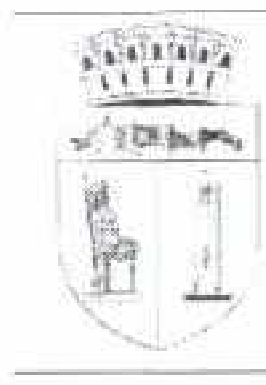
\includegraphics[height=1.5cm]{assets/stema-cluj.png}%
\hspace{0.2cm}%
\raisebox{0.5cm}{\parbox[t]{3.5cm}{\textbf{PRIMĂRIA}\\\textbf{CLUJ-NAPOCA}}}
\end{minipage}%
\begin{minipage}[t]{0.30\textwidth}
\centering
\vspace{0.25cm}

\includegraphics[width=5cm]{assets/barcode-491001.png}
\end{minipage}%
\begin{minipage}[t]{0.30\textwidth}
\raggedleft
\vspace{0.6cm}
Nr. \fillline[3cm] / \fillline[1cm]
\end{minipage}

\vspace{0.3cm}
\hrule
\vspace{0.3cm}

\begin{center}
\textbf{CERERE}\\
\textit{actualizare date cu caracter personal -- persoană fizică}
\end{center}

\vspace{0.3cm}

\textbf{CĂTRE}\\
\textit{MUNICIPIUL CLUJ-NAPOCA}\\
\textit{DIRECȚIA IMPOZITE ȘI TAXE LOCALE}\\
\textit{SERVICIUL CONSTATARE, IMPUNERE, CONTROL PERSOANE FIZICE}\\
\textit{e-mail:} \underline{registratura@primariaclujnapoca.ro}

\vspace{0.25cm}

\textbf{I. CONTRIBUABIL}\\
Nume/Prenume \underline{ {{nume_complet}} }, \textbf{CNP/CIF/NIF} \underline{ {{cnp}} },\\
\textbf{IDENTIFICAT(Ă)} cu Actul \underline{ C.I. }, Seria \underline{ {{ci_seria}} }, Nr. \underline{ {{ci_numar}} }, \textbf{DOMICILIUL} în Localitatea\\
\underline{ {{localitate}} }, Str. \underline{ {{strada}} }, Nr. \underline{ {{numar}} }, Bl. \underline{ {{bloc}} }, Ap. \underline{ {{apartament}} }, Jud./Sect. \underline{ {{judet}} },\\
\textbf{TELEFON} \underline{ {{telefon}} }, \textbf{E-MAIL} \underline{ {{email}} }, \textbf{ADRESA DE CORESPONDENȚĂ} \underline{ {{adresa_corespondenta}} }

\vspace{0.25cm}

\textbf{II. SOLICIT ACTUALIZAREA DATELOR CU CARACTER PERSONAL.}\\
\textbf{ATAȘEZ ACTUL DE IDENTITATE\textsuperscript{1}}

\vspace{0.3cm}

\textbf{Tip modificare:} \underline{ {{tip_modificare}} }\\
\textbf{Date noi:} \underline{ {{date_actualizate}} }

\vspace{0.25cm}

\textbf{III. DATA}\\
\underline{ {{data_cerere}} }

\vspace{0.25cm}

\textbf{IV. SEMNĂTURA}\\
\hrulefill

\vspace{0.25cm}

\hrule

\vspace{0.3cm}

\scriptsize
\textsuperscript{1} Primăria municipiului Cluj-Napoca asigură gratuit fotocopierea documentelor.\\
Pentru documentele emise de către alte instituții publice, organe de specialitate ale administrației publice centrale și locale, precum și persoane juridice de drept privat, care potrivit legii au obținut statut de utilitate publică sau sunt autorizate să presteze un serviciu public, în regim de putere publică, pe care solicitantul nu le depune, acesta are posibilitatea de a-și da consimțământul expres ca Primăria municipiului Cluj-Napoca să obțină în numele său copii sau extrase ale acestora.

\vspace{0.25cm}

\begin{minipage}[t]{0.65\textwidth}
www.primariaclujnapoca.ro\\
telefon: 0264/596.030\\
Cluj-Napoca, str. Moţilor, nr. 3
\end{minipage}%
\begin{minipage}[t]{0.35\textwidth}
\raggedleft

\includegraphics[width=4cm]{assets/barcode-491001.png}
\end{minipage}

\vspace{0.3cm}

Timp estimativ de completare: 10 minute

\vspace{0.2cm}

Datele personale care vă sunt solicitate prin prezenta cerere vor fi prelucrate numai în vederea procesării și soluționării solicitării dumneavoastră. Primăria municipiului Cluj-Napoca garantează securitatea procesării datelor și arhivarea acestora în conformitate cu prevederile legale în vigoare. Responsabilul Primăriei municipiului Cluj-Napoca cu protecția datelor poate fi contactat pe adresa de email dpo@primariaclujnapoca.ro.

În conformitate cu Regulamentul nr. 679/2016 aveți dreptul de a solicita Primăriei municipiului Cluj-Napoca, în ceea ce priveşte datele cu caracter personal referitoare la persoana vizată, accesul la acestea, rectificarea sau ştergerea acestora sau restricţionarea prelucrării sau a dreptului de a vă opune prelucrării, precum şi a dreptului la portabilitatea datelor.

\end{document}
